%% if you are submitting an initial manuscript then you should have submission as an option here
%% if you are submitting a revised manuscript then you should have revision as an option here
%% otherwise options taken by the article class will be accepted
\documentclass[submission]{FPSAC2021}
%% but DO NOT pass any options (or change anything else anywhere) which alters page size / layout / font size etc

%% note that the class file already loads {amsmath, amsthm, amssymb}



\allowdisplaybreaks
\usepackage[bottom]{footmisc}
% \usepackage{amssymb,amsmath,amsthm}
\usepackage{caption}
\usepackage{subcaption}
\usepackage{amsbsy,algpseudocode,ragged2e,graphicx,framed,bm,soul,xcolor,enumitem,tabularx,multicol,mathtools,fancyhdr,setspace,tikz,listings,ytableau, float, microtype,ulem,scrextend, wrapfig}
\usepackage[plain]{algorithm}
\usepackage[vcentermath,enableskew]{youngtab}
% \usepackage[colorlinks=true, pdfstartview=FitV, linkcolor=blue, citecolor=blue, urlcolor=blue]{hyperref}
\usepackage{chngcntr}
\usepackage{enumitem}
\usetikzlibrary{arrows,matrix}
\definecolor{purple}{RGB}{118, 37, 138}
\definecolor{dgreen}{RGB}{5, 125, 45}
\usepackage[many]{tcolorbox}
\usepackage[justification=centering]{caption}
%\vbadness=10000
\usepackage{etoolbox}
\usepackage{tikz}
\usetikzlibrary{tikzmark}
\usetikzlibrary{calc}

\errorcontextlines\maxdimen

\normalem

    \algblockdefx[customBlk]{Begin}{End}
  {\textbf{begin} }
  {\textbf{end} }
  \algnewcommand{\LineComment}[1]{\State \hspace{0.5 em} \(\blacktriangleright\) #1}
  \newlength{\whilewidth}
\settowidth{\whilewidth}{\algorithmicwhile\ }
\algrenewcommand{\algorithmiccomment}[1]{\hspace{0.33em}$\blacktriangleright$ #1}
%\usepackage[nottoc,notlot,notlof]{tocbibind}
\makeatletter
\newtheorem*{rep@theorem}{\rep@title}
\newcommand{\newreptheorem}[2]{%
\newenvironment{rep#1}[1]{%
 \def\rep@title{#2 \ref{##1}}%
 \begin{rep@theorem}}%
 {\end{rep@theorem}}}
\makeatother
\theoremstyle{plain}
\newtheorem{theorem}{Theorem}[section]
\newtheorem{lemma}[theorem]{Lemma}
\newtheorem{conjecture}[theorem]{Conjecture}
\newtheorem{proposition}[theorem]{Proposition}
\newtheorem{corollary}[theorem]{Corollary}
\theoremstyle{definition}
\newtheorem{algo}[theorem]{Algorithm}
\newtheorem{definition}[theorem]{Definition}
\newtheorem{example}[theorem]{Example}
\newtheorem{remark}[theorem]{Remark}
\numberwithin{equation}{section}
\counterwithout{figure}{section}
\newreptheorem{theorem}{Theorem}
\newreptheorem{conjecture}{Conjecture}
\newreptheorem{lemma}{Lemma}
\newreptheorem{corollary}{Corollary}
\newreptheorem{remark}{Remark}
%%% END PACKAGES %%%}

%%% MACROS %%%{


% begin vertical rule patch for algorithmicx (http://tex.stackexchange.com/questions/144840/vertical-loop-block-lines-in-algorithmicx-with-noend-option)
\makeatletter
% start with some helper code
% This is the vertical rule that is inserted
\newcommand*{\algrule}[1][\algorithmicindent]{\makebox[#1][l]{\hspace*{.5em}\vrule height .5\baselineskip depth .25\baselineskip}}%

\newcount\ALG@printindent@tempcnta
\def\ALG@printindent{%
    \ifnum \theALG@nested>0% is there anything to print
        \ifx\ALG@text\ALG@x@notext% is this an end group without any text?
            % do nothing
            \addvspace{-3pt}% FUDGE for cases where no text is shown, to make the rules line up
        \else
            \unskip
            % draw a rule for each indent level
            \ALG@printindent@tempcnta=1
            \loop
                \algrule[\csname ALG@ind@\the\ALG@printindent@tempcnta\endcsname]%
                \advance \ALG@printindent@tempcnta 1
            \ifnum \ALG@printindent@tempcnta<\numexpr\theALG@nested+1\relax% can't do <=, so add one to RHS and use < instead
            \repeat
        \fi
    \fi
    }%
\usepackage{etoolbox}
% the following line injects our new indent handling code in place of the default spacing
\patchcmd{\ALG@doentity}{\noindent\hskip\ALG@tlm}{\ALG@printindent}{}{\errmessage{failed to patch}}
\makeatother
% end vertical rule patch for algorithmicx



\renewcommand{\th}{$^\text{th}$ }
%\renewcommand{\st}{$^\text{st}$ }
\newcommand{\ub}[1]{\overline{#1}}
\newcommand{\lb}[1]{\underline{#1}}
%\renewcommand{\rd}{$^\text{rd}$ }
\newcommand\Warning{%
 \makebox[1.4em][c]{%
 \makebox[0pt][c]{{{\color{red}\textbf{!}}}}%
 \makebox[0pt][c]{\raisebox{-.4em}{\color{red}\Huge$\bigtriangleup$}}}}%
\newcommand{\inv}{^{-1}}
\newcommand{\meq}{\overset{\text{must}}{=}}
\newcommand{\bv}[2]{\begin{bmatrix}#1\\#2\end{bmatrix}}
\newcommand\bvv[1]{\setstackEOL{,}\bracketVectorstack{#1}}
\newcommand{\bvvv}[3]{\begin{bmatrix}#1\\#2\\#3\end{bmatrix}}
\newcommand{\stab}{\text{Stab}}
\newcommand{\orb}{\text{Orb}}
\newcommand{\inr}{\in \mathbb{R}}
\newcommand{\mt}[4]{\begin{bmatrix}#1&#2\\#3&#4\end{bmatrix}}
\newcommand{\inz}{\in \mathbb{Z}}
\newcommand{\inn}{\in \mathbb{N}}
\newcommand{\inc}{\in \mathbb{C}}
\newcommand{\la}{\langle}
\newcommand{\ra}{\rangle}
\newcommand{\Z}{\mathbb{Z}}
\newcommand{\R}{\mathbb{R}}
\newcommand{\C}{\mathbb{C}}
\newcommand{\Q}{\mathbb{Q}}
\newcommand{\N}{\mathbb{N}}
\DeclareMathOperator{\id}{id}
\DeclareMathOperator{\sh}{sh}
\DeclareMathOperator{\sgn}{sgn}
\DeclareMathOperator{\SDself}{SD}
\DeclareMathOperator{\SShself}{sh}
\DeclareMathOperator{\Ptself}{P}
\DeclareMathOperator{\lcm}{lcm}
\newcommand{\Ci}[1]{\overset{#1}{\scalebox{.8}{C}}}
\newcommand{\CommentStart}{\Iffalse}
\newcommand{\CommentEnd}{\fi}
\newcommand{\SD}[1]{\SDself(#1)}
\renewcommand{\P}[1]{\Ptself(#1)}
\newcommand{\Sh}[1]{\SShself#1}
\newcommand{\SSh}[1]{\SShself#1}
\newcommand\allbold[1]{{\boldmath\textbf{#1}}
}\newcommand{\doi}[1]{\href{http://dx.doi.org/#1}{\texttt{doi:#1}}}
\newcommand{\arxiv}[1]{\href{http://arxiv.org/abs/#1}{\texttt{arXiv:#1}}}
\newcommand{\inner}[2]{\left\langle #1, #2 \right\rangle} 
\newcommand{\innernoscale}[2]{\langle #1, #2 \rangle} % inner product but does not scale the brackets

\newcommand{\splitAlg}[1]{\algstore{#1}
\end{algorithmic}
\end{algorithm}
\begin{algorithm}[H]
\begin{algorithmic}[1]
\algrestore{#1}}

%% define your title in the usual way
\title%[Box-ball systems and RSK tableaux]
{Box-ball systems and RSK tableaux}

%% define your authors in the usual way
%% use \addressmark{1}, \addressmark{2} etc for the institutions, and use \thanks{} for contact details

\author[B.~Drucker, E.~Garcia, E.~Gunawan, and R.~Silver]{Ben Drucker\addressmark{1}, Eli Garcia\addressmark{2}, Emily Gunawan\addressmark{3}, and Rose Silver\addressmark{4}
}

%% then use \addressmark to match authors to institutions here
\address{\addressmark{1}Swarthmore College, Swarthmore, PA, USA \\ 
\addressmark{2}Massachusetts Institute of Technology, Cambridge, MA, USA\\
\addressmark{3}Department of Mathematics, University of Oklahoma, Norman, OK, USA
\\
\addressmark{4}Northeastern University, Boston, MA, USA}


%% put the date of submission here
\received{\today}

%% leave this blank until submitting a revised version
%\revised{}

%% please don't use custom commands in your abstract / resume, as these will be displayed online
%% likewise for citations -- please don't use \cite, and instead write out your citation as something like (author year)
\abstract{A box-ball system is a collection of discrete time states. At each state, we have a collection of countably many boxes with each integer from $1$ to $n$ assigned to a unique box; 
the remaining boxes are considered empty. 
A permutation on $n$ objects gives a box-ball system state by assigning the permutation in one-line notation to the first $n$ boxes. 
After a finite number of steps, the system will reach a so-called soliton decomposition which has an integer partition shape. 
We prove the following: if the soliton decomposition of a permutation is a standard Young tableau or if its shape coincides with its Robinson--Schensted (RS) partition, 
then its soliton decomposition and its RS insertion tableau 
are equal. 
We study the time required for a box-ball system to reach a steady state. We also generalize Fukuda's single-carrier algorithm to algorithms with
more than one carrier. 
}

%% put your French abstract here, or comment this out if you don't have one
% \resume{\lipsum[2]}

%% put your keywords here, or comment this out if you don't have them yet
 \keywords{box-ball system,
RSK correspondence,
% Robinson--Schensted--Knuth correspondence,
tableaux, Greene's theorem
}

%% you can include your bibliography however you want, but using an external .bib file is STRONGLY RECOMMENDED and will make the editor's life much easier
%% regardless of how you do it, please use numerical citations, ie. [xx, yy] in the text

%% this sample uses biblatex, which (among other things) takes care of URLs in a more flexible way than bibtex
%% but you can use bibtex if you want
\usepackage[backend=bibtex]{biblatex}
\addbibresource{bib.bib}
%% note the \printbibliography command at the end of the file which goes with these biblatex commands

\begin{document}

\maketitle
%% note that you DO NOT have to put your abstract here -- it is generated by \maketitle and the \abstract and \resume commands above

%\tableofcontents

\section{Introduction}
    A \emph{box-ball system} (BBS) is a collection of discrete time states. At each state, we have a collection of countably many boxes with each integer from $1$ to $n$ assigned to a unique box; the remaining boxes are considered ``empty.'' A permutation $\pi \in S_n$ gives a box-ball system state by assigning the permutation in one-line notation to the first $n$ boxes. We apply a \emph{BBS move} in the forward direction (letting time $t$ increase by 1) by moving each integer from smallest to largest to the nearest empty space to its right. 
    See Figure \ref{fig: intro to BBS}.
\begin{figure}[H]
    \centering
    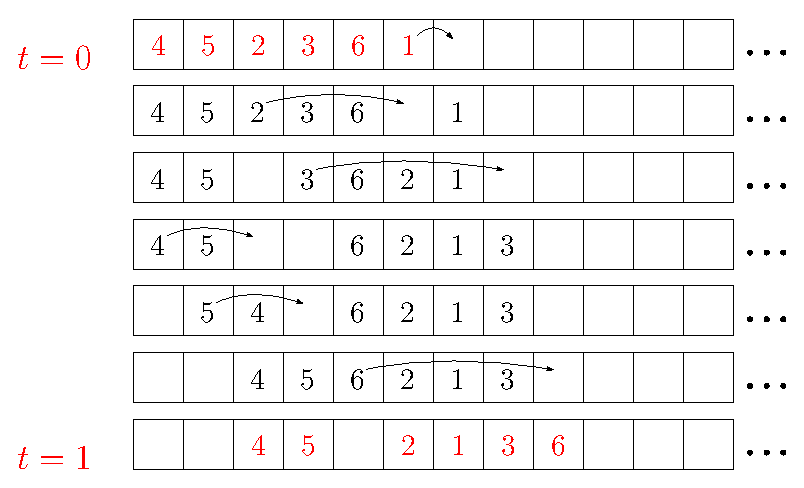
\includegraphics[width = 0.41\textwidth]{Step3.eps}
    \caption{Performing a forward BBS move on $\pi=452361$}
    \label{fig: intro to BBS}
\end{figure}

A \emph{soliton} is a consecutive increasing sequence which is preserved by all subsequent BBS moves. After a finite number of BBS moves, a box-ball system containing a configuration $\pi$ will reach a \emph{steady state},  
decomposing into solitons
whose sizes are weakly increasing from left to right, 
that is, forming an integer partition shape~\cite{Takahashi93}. 
See Figure \ref{fig: BBS steady state}.
    \begin{figure}[H]
    \centering
    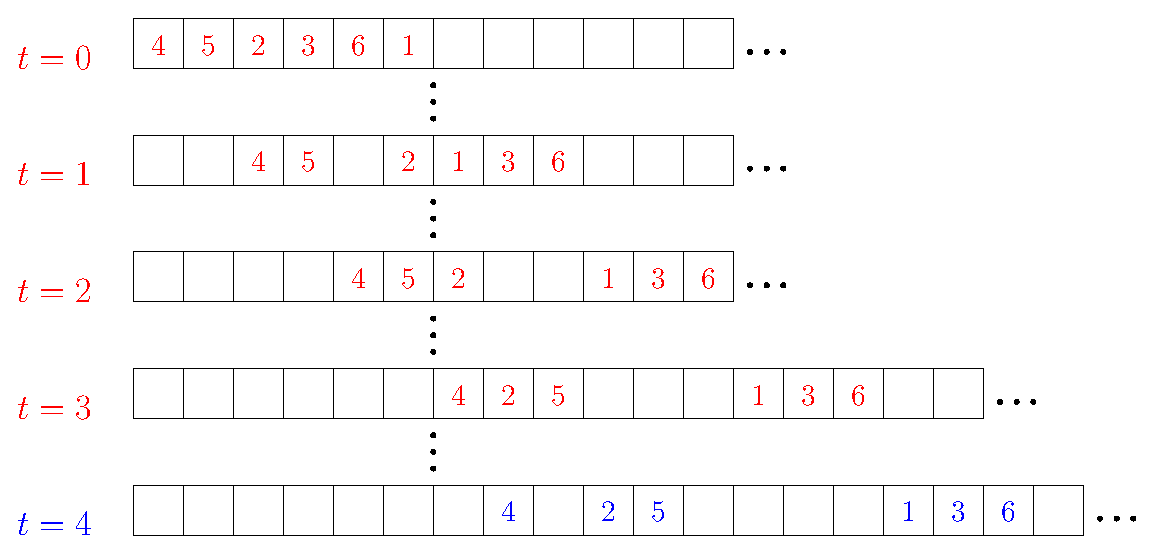
\includegraphics[width = 0.65\textwidth]{Step4V2.eps}
    \caption{Forward BBS moves for $\pi=452361$. Steady state is first achieved at $t=3.$} 
    \label{fig: BBS steady state}
\end{figure}

From such a state, 
we can construct 
the \emph{soliton decomposition} of a permutation, denoted SD, 
by stacking solitons.
We obtain a tableau where each row is increasing but which may or may not be standard. 
For example, the  soliton decomposition of the box-ball system containing  $\pi=452361$ shown in Figure~\ref{fig: BBS steady state} is \[
{\small  \SD{\pi}=
    ~
    \young(136,25,4)}. 
    \]

\par The well-known Robinson--Schensted (RS) insertion algorithm is 
a bijection \\
${\pi \mapsto (\P{\pi},Q(\pi))}$
from $S_n$ onto pairs of standard Young tableaux of size $n$, see~\cite{Sch61}.
The tableau $\P{\pi}$ is called the \emph{insertion tableau} of $\pi$, and the tableau $Q(\pi)$ is called the \emph{recording tableau} of $\pi$. 

The \emph{reading word} of a % (not-necessarily standard)
Young tableau is the permutation formed by concatenating the rows of the tableau from bottom to top. 
If $r$ is the reading word of a standard Young tableau $T$, then $P(r)=T$. 

For example, 
if $\pi=452361$, then 
\[
\P{\pi}=\young(136,25,4), 
~~
Q(\pi)=\young(125,34,6).
\]
The tableau  {$\P{\pi}$} 
has reading word $r=425136$, and
the insertion tableau of $r$ is the tableau $\P{\pi}$. 


\subsection{BBS soliton partition and localized version of  Greene's theorem}
\label{sec:local Greene's theorem}
\label{sec: BBS soliton proofs}

 Greene famously 
showed that the RS partition of a permutation and its conjugate record the numbers of disjoint unions of increasing and decreasing  sequences of the permutation~\cite[Theorem ~3.1]{Gre74}.  
 Lewis, Lyu, Pylyavskyy, and Sen recently 
showed that 
the partition shape of the soliton decomposition 
 of a permutation and its conjugate 
record 
a pair of similar collections of permutation statistics~\cite[Lemma 2.1]{LLPS19}. 
They studied an alternate version of the box-ball system, so we reframe their result to match our box-ball convention.



\begin{definition}
\label{defn: lambda and mu}
    For $\pi = \pi_1\cdots\pi_n\in S_n$ and $k\geq 1,$ we define \[
    I_k = \max_{\pi=u_1\mid\cdots\mid u_k}\sum_{j=1}^k i(u_j), \]
    where $i(u_j)$ is the length of the longest increasing subsequence in $u_j$ and the maximum is taken over ways of writing $\pi$ as a concatenation $u_1 \mid \dots \mid u_k$ of consecutive subsequences. 
    That is, we consider all ways to break $\pi$ into $k$ consecutive subsequences, sum the $i(u_j)$ values for each way, and let $I_k$ be the maximum sum. 
    We also define 
    \[ D_k = \max_{\pi= u_1 \sqcup \cdots \sqcup u_k} \sum_{j=1}^k d(u_j),\] where $d(u_j)= 1+|\{$descents in $u_j\}|$ 
    and the maximum is taken over
    ways to write $\pi$ as the union of 
    disjoint subsequences $u_i$ of $\pi$. 
    Notice that we only require $u_1,\dots, u_k$ to be disjoint, \emph{not} consecutive. We then form the sequences $$\lambda_{BBS}(\pi) = (I_1,I_2-I_1,I_3-I_2,\dots) ~ \text{ and } ~ \mu_{BBS}(\pi) = (D_1,D_2-D_1,D_3-D_2,\dots).$$
\end{definition}


\begin{lemma}[Corollary of {\cite[Lemma 2.1]{LLPS19}}]
\label{Lem: R_k gives SD shape}
        If $\pi\in S_n$, then  the shape $\sh \SD \pi$ of $\SD\pi$ is equal to $\lambda_{BBS}(\pi).$ Furthermore, the  conjugate of $\sh\SD\pi$ is equal to $\mu_{BBS}(\pi).$
\end{lemma}
        
        
For example, let $\pi = 521643$. Then $\lambda_{BBS}(\pi)=(2,1,1,1,1)$ and $\mu_{BBS}(\pi)=(5,1)$. The soliton decomposition $\SD{\pi}$ is the (non-standard) tableau given in Figure \ref{fig: SDpi}. 

\subsection{When the soliton decomposition and RS insertion tableau coincide}

We show that reading words of standard tableaux have well-behaved soliton decomposition. 

\begin{theorem}
\label{Thm: forwards t = 0}
A permutation $r$ reaches its soliton decomposition at time $t=0$ if and only if $r$ is the reading word of a standard Young tableau. 
In particular, if $r$ is the reading word of a standard tableau $T$, then $\SD{r}=T$ and so $\SD{r}=T=\P{r}$. 
\end{theorem}


In Section \ref{sec: skew}, we generalize Theorem \ref{Thm: forwards t = 0} to standard skew tableaux. 

In general, the soliton decomposition and the RS insertion tableau of a permutation do not coincide.
Surprisingly, having a standard tableau for a soliton decomposition 
or having a soliton decomposition shape which equals the RS partition shape 
is enough to guarantee that the soliton decomposition and the RS insertion  tableau coincide.

\begin{theorem}\label{thm:tfae} 
Suppose $\pi$ is a permutation. Then 
    the following are equivalent:
    \begin{enumerate}
        \item\label{tfae:itm:one} 
        $\SD{\pi} = \P{\pi}.$
        \item\label{tfae:itm:two} 
        $\SD{\pi}$ is a standard tableau.
        \item \label{tfae:itm:three}
        The shape of $\SD{\pi}$ equals the shape of $\P{\pi}$.
    \end{enumerate}
    \end{theorem}
 See Section \ref{sec:proof of tfae} for a proof of Theorem \ref{thm:tfae}. 
 The proof that  (\ref{tfae:itm:three}) implies (\ref{tfae:itm:two}) 
 was suggested to the authors by Darij Grinberg. 

\subsection{Three types of Knuth moves}

The RS insertion tableau is preserved under any Knuth move~\cite{Knuth70}. 
In contrast, the soliton decomposition is only  preserved under certain types of Knuth moves. 

\begin{definition}[Knuth Moves]
       Suppose $\pi$, $\sigma \in S_n$ and $x<y<z$.
            \begin{itemize}
                \item $\pi$ and $\sigma$ differ by a Knuth relation of the \textbf{first kind} ($K_1$) if %\vspace{-.5em}
                \begin{center}
                $\pi=\pi_1 \dots \textcolor{black}{y}\textcolor{black}{x}\textcolor{black}{z} 
                \dots \pi_n$
                and
                $\sigma=\pi_1 \dots \textcolor{black}{y}\textcolor{black}{z}\textcolor{black}{x} \dots \pi_n$ 
                %\vspace{-.5em}
                \end{center} 
                
                \item $\pi$ and $\sigma$ differ by a Knuth relation of the \textbf{second kind} ($K_2$) if \begin{center}
                %\vspace{-.5em}
                $\pi=x_1 \dots \textcolor{black}{x}\textcolor{black}{z}\textcolor{black}{y} \dots x_n$ and $\sigma=x_1 \dots \textcolor{black}{z}\textcolor{black}{x}\textcolor{black}{y} \dots x_n$
                %\vspace{-.5em}
                \end{center}  
                
                \item $\pi$ and $\sigma$ differ by Knuth relations of \textbf{both kinds} ($K_B$) if \begin{center} 
                %\vspace{-.5em}
                $\pi=x_1 \dots \textcolor{black}{y_1}\textcolor{black}{x}\textcolor{black}{z}\textcolor{black}{y_2} \dots x_n$ and $\sigma=x_1 \dots \textcolor{black}{y_1}\textcolor{black}{z}\textcolor{black}{x}\textcolor{black}{y_2} \dots x_n$ %\vspace{-.75em}
                \end{center}
        where 
         $x<y_1<z$ and  $x<y_2<z$.
        \end{itemize}
\end{definition}


Using the localized version of Greene's Theorem 
given in Section \ref{sec:local Greene's theorem}, 
we prove a partial characterization of 
  the shape of 
  $\SDself$  
in terms of types of Knuth moves.


\begin{theorem}\label{thm: knuth paths}
If $\pi$ and $w$ are related by a sequence of $K_1$ or $K_2$ moves (but not $K_B$), then $\sh\SD{\pi}=
\sh\SD{w}$. 
If $\pi$  and $w$ are related by a sequence of Knuth moves containing an odd number of $K_B$ moves, then $\sh \SD{\pi}
\neq
\sh\SD{w}$. 
\end{theorem} 


    
This allows us to use Knuth moves to find more  permutations whose soliton decomposition and RS insertion tableau coincide.
    

\begin{corollary}[Corollary of
Theorem~\ref{thm:tfae}
and 
Theorem~\ref{thm: knuth paths}]
\label{cor: follows directly}
If $\pi\in S_n$ is a sequence of $K_1$ or $K_2$ moves (but not $K_B$) away from the reading word of a standard tableau $T$, 
then $\SD{\pi}=\P{\pi}=T.$ 
If $\pi\in S_n$ is related to the reading word of a standard tableau by a sequence of Knuth moves such that an odd number of the moves are $K_B$ moves, 
 then $\SD{\pi}\neq \P{\pi}=T$.
\end{corollary}

\begin{proposition}
Suppose $\pi\in S_n$ is the reading word of a standard tableau. Let $\pi'$ be a permutation one $K_1$ or $K_2$ (but not $K_B$) move away from $\pi$. Then $\pi'$ reaches a steady state after one BBS move.  
\end{proposition}



\section{Steady states}

We study the steady-state configurations and the minimum time-steps to go from a permutation to its 
% (forward) 
soliton decomposition.  

\subsection{Standard tableaux of skew shapes}
\label{sec: skew}
A BBS state can be represented as an array containing the integers from 1 to $n$ as follows: scanning the boxes from right to left, each string of increasing integers becomes a row in the array. 
A string of $k$ empty boxes indicates that the next row below should be shifted $k$ steps to the left.
Note that this array has increasing rows but not necessarily increasing columns; it also may not have a valid skew shape. The following is a generalization of Theorem \ref{Thm: forwards t = 0}.
\begin{theorem}\label{thm: t=0 generalization} A BBS configuration $C$ is in steady state if and only if the associated array is a standard skew tableau whose rows are weakly decreasing in length. \end{theorem}
\begin{example}[of Theorem \ref{thm: t=0 generalization}]
Let $\pi = 521643$. The soliton decomposition $\SD{\pi}$ is the tableau given in Figure \ref{fig: SDpi}. Note that $C=e52e6413ee\dots$ is a steady-state configuration (at $t=1$), where we represent empty boxes with the symbol $e$.
The configuration $C$
yields the standard skew tableau in Figure \ref{fig:resultantSkew}.
Conversely, if given the skew tableau in Figure \ref{fig:resultantSkew}
(with no knowledge of the original permutation), we may conclude the corresponding BBS configuration, $52e6413$, is in steady state.

\begin{figure}[H]
\centering
\begin{minipage}{.4\textwidth}
  \centering
    $\raisebox{-2em}{\scalebox{.85}{\young(13,4,6,2,5)}}$
  \captionof{figure}{$\SD{\pi}$}
  \label{fig: SDpi}
\end{minipage}%
\begin{minipage}{.6\textwidth}
  \centering
  $\scalebox{.85}{\young(:13,:4,:6,2,5)}$
  \captionof{figure}{
  Skew tableau for $C=e52e6413ee\dots$ 
  }
  \label{fig:resultantSkew}
\end{minipage}
\end{figure}
\end{example}
\subsection{Permutations with \textit{n--}3 time steps} 


We also study the relationship between the RS recording tableau of a permutation and the behavior of its box-ball system.

\begin{definition}\label{def: Q_0}
If $n \geq 5$, let $Q_0:=Q_0(n)$ denote the tableau $$\begin{ytableau}
 1 & 2 &\none[\hdots]&\scalebox{.5}{$n-2$}&\scalebox{.5}{$n-1$}\\
 3 & 4\\
 n
 \end{ytableau}.$$
Let $S_n(Q_0)$ be the set of permutations $\pi \in S_n$ such that its recording tableau $Q(\pi)$ is equal to $Q_0$.
\end{definition}


\begin{example}
For $n=5$, the five permutations of this set are the following.
\begin{multicols}{5}
 45132
 
 25143
 
 35142
 
 45231
 
 35241
\end{multicols}
For $n=6$, the sixteen permutations of this set are as follows.
\begin{multicols}{8}
\noindent 451362
251463
351462
452361
352461
561243
261354
361254
461253
561342
261453
361452
461352
562341
362451
462351
\end{multicols}
\end{example}

 \begin{remark}
It follows from Definition \ref{def: Q_0} that the RS algorithm induces a bijection from $S_n(Q_0)$ to the set of standard tableaux of shape $(n-3,2,1)$, see~\cite{Lang02OEIS}.
 \end{remark}

We define the \emph{steady-state value} of a permutation $\pi$ to be the minimum number of BBS moves required to go from $\pi$ to a steady state. 

\begin{proposition}
    Every permutation in $S_n(Q_0)$ has steady-state value of $n-3.$
\end{proposition}
The following conjecture has been computationally verified up to $n=10.$
\begin{conjecture}
     A permutation not in $S_n(Q_0)$ has steady-state value smaller than $n-3$.
\end{conjecture}

\section{Proof of Theorem \ref{thm:tfae}}
\label{sec:proof of tfae}
\subsection{Fukuda's carrier algorithm as a sequence of Knuth moves}\label{sec: carrier alg bg}
Some of our proofs use an algorithm called 
the \emph{carrier algorithm}  
which was first introduced in~\cite{TM97carrier} 
and generalized in~\cite[Section~3.3]{fukuda04}.
It is used to calculate the $t=k+1$ state of a box-ball system given the $t = k$ state.


Let $B$ be a box-ball configuration. By convention, let $e\coloneqq n+1$. 
Fill a \emph{carrier} (a sequence of $n$ weakly increasing entries) with $n$ copies of $e$. 
We begin the insertion process (Process 1) by putting $B$ to the right of the carrier. We insert $p$, the leftmost element of $B$, into the carrier.
Let $s$ be the smallest entry in the carrier greater than $p$ if such entry exists. We replace $s$ by $p$ and eject $s$ from the carrier, placing it to the left of the carrier. If no entry greater than $p$ exists in the carrier, we eject the smallest element in the carrier, and put $p$ in the rightmost location of the carrier.
We continue inserting elements of $B$ in this manner until all non-$e$ entries of $B$ have been inserted into the carrier. 
Next, we begin the flushing process (Process 2). We eject all non-$e$ elements in the carrier (in increasing order) by inserting $e$'s into the carrier. This concludes one application of the carrier algorithm. The string of elements to the left of the carrier is the result of performing one box-ball move on $B$.

\begin{example}[Carrier Algorithm~\cite{fukuda04}] 
We compute the $t=3$ configuration of the box-ball system from Figure \ref{fig: BBS steady state} by applying the carrier algorithm to the $t=2$ configuration. We set $B\coloneqq eeee452ee136\dots$. 
The carrier algorithm then proceeds as follows:
    \begin{multicols}{2}
    \begin{minipage}[H]{0.45\textwidth}
            \begin{center}
            \textbf{begin} Process 1: insertion process
            \vspace{-1em}
            \end{center}
            \begin{align*}
        &\underbracket{eeeeee}eeee452ee136\\
        e&\underbracket{eeeeee}eee452ee136\\
        &\vdots\\%[-2mm]
        eeee&\underbracket{eeeeee}452ee136\\
        eeeee&\underbracket{4eeeee}52ee136\\
        eeeeee&\underbracket{45eeee}2ee136\\%[-2mm]
        eeeeee4&\underbracket{25eeee}ee136\\
        eeeeee42&\underbracket{5eeeee}e136\\
        eeeeee425&\underbracket{eeeeee}136\\
        &\vdots\\%[-2mm]
        eeeeee425eee&\underbracket{136eee}
        \end{align*}
        \begin{center}
            \textbf{end} insertion process
            \end{center}
            \end{minipage}
            \begin{minipage}[H]{0.45\textwidth}
            \begin{center}
            \textbf{begin} Process 2: flushing process
            \vspace{-1em}
            \end{center}
        \begin{align*}
        eeeeee425eee&\underbracket{136eee}\leftarrow e\\
        eeeeee425eee1&\underbracket{36eeee}\leftarrow e\\
        eeeeee425eee13&\underbracket{6eeeee}\leftarrow e\\
        eeeeee425eee136&\underbracket{eeeeee}
        \end{align*}
        \begin{center}
            \textbf{end} flushing process
        \end{center}
        \end{minipage}
\end{multicols}
After each insertion, the sequence in the carrier is weakly increasing.
\end{example}

    
    \begin{remark}[{\cite[Remark 4]{fukuda04}}]\label{rmk: carrier is knuth}
        The carrier algorithm can be viewed as a sequence of Knuth moves.  
        Consider the insertion of $p$ into the carrier. 
         If the carrier contains a number greater than $p$, then the insertion process is equivalent to applying a sequence of $K_1$ moves
        \begin{center}
            $\underbracket{\cdots s z_1\cdots z_{l-1}z_l} \: p$ \\
            $\underbracket{\cdots s z_1\cdots z_{l-1} p z_l}$ \\%[-1mm]
            $\vdots$ \\%[-1mm]
            $\underbracket{\cdots s pz_1\cdots z_{l-1}z_l}$
        \end{center}
        followed by a sequence of $K_2$ moves:
        \begin{center}
         $\underbracket{x_1\cdots x_{m-1}x_m s p\cdots}$ \\[2mm]
            $\underbracket{x_1\cdots x_{m-1}s x_mp\cdots}$ \\%[-1mm]
            
            $\vdots$ \\%[-1mm]
            $s \underbracket{x_1\cdots x_{m-1}x_mp\cdots}.$
        \end{center}
        Otherwise, if $p$ is greater than or equal to every element in the carrier, we apply the trivial transformation:
        \vspace{-5mm}
           \begin{align*} &\underbracket{x\cdots}\: p \\
          x\:&\underbracket{\cdots p}.
        \end{align*}
    \end{remark}
    
    \begin{lemma}
    [{\cite[Theorem 3.1]{fukuda04}}]
    \label{lemma:preserved}
    The RS insertion tableau is a conserved quantity under the time evolution of the box-ball system, that is, it is preserved under each BBS move.
    \end{lemma}
    
    
    \subsection{Soliton decompositions and RSK tableaux}



The following gives a characterization of permutations whose soliton decompositions are equal to their RS insertion tableaux.




\begin{reptheorem}{thm:tfae} 
Let $\pi$ be a permutation. Then 
the following are equivalent:
    \begin{enumerate}
        \item 
        $\SD{\pi} = \P{\pi}.$
        \item 
        $\SD{\pi}$ is a standard tableau.
        \item 
        the shape of $\SD{\pi}$ equals the shape of $\P{\pi}$.
    \end{enumerate}
    \end{reptheorem}

\begin{lemma}[Due to Darij Grinberg]
\label{lem: Grinberg}
Suppose $S$ is a row-strict tableau of a partition, that is, every row is increasing (with no restrictions on the columns). 
Let $r$ be the reading word of the tableau $S$.
Let $\P{r}$ be the RS insertion tableau of $r$. 
If the shape of $S$ equals the shape of $\P{r}$, then $S$ is standard.
\end{lemma}

\begin{proof}[Proof of Theorem \ref{thm:tfae}.]
Certainly \eqref{tfae:itm:one} implies \eqref{tfae:itm:two} and \eqref{tfae:itm:three}. First, we show that (\ref{tfae:itm:two}) implies (\ref{tfae:itm:one}). Suppose that $\SD{\pi}$ is a standard tableau. Let $r$ denote the reading word of $\SD{\pi}.$ We know that $r$ is the order in which the elements of $\pi$ are configured once we reach a steady state. 
By Lemma \ref{lemma:preserved}, $\P{\pi} = \P{r}.$
Since $r$ is the reading word of $\SD{\pi},$ a standard tableau, we have $\P{r} = \SD{\pi}$ by Theorem \ref{Thm: forwards t = 0}. 
Therefore $\P{\pi}=\SD{\pi}$.
        
Next, we show that  \eqref{tfae:itm:three} implies  \eqref{tfae:itm:two}. Suppose that the shape of $\SD{\pi}$ equals the shape of $\P{\pi}$. Let $r$ be the reading word of $\SD{\pi}$. 
Lemma~\ref{lemma:preserved} 
tells us that the RS insertion tableau is preserved under a sequence of box-ball moves, so $\P{\pi}=\P{r}$ and, in particular, $\text{sh}\P{\pi}=\text{sh}\P{r}$. By assumption, we have  $\text{sh}\SD{\pi}=\text{sh}\P{r}$. Since $\SD{\pi}$ is a row-strict tableau and $r$ is the reading word of $\SD{\pi}$, Lemma \ref{lem: Grinberg} tells us that $\SD{\pi}$ is standard.
\end{proof}
    



\section{Multi-carrier  algorithms}

In this section, we give insertion algorithms that can help us study steady states and soliton decompositions.

\subsection{M-carrier algorithm}\label{sec: m-carrier}

 
In this section, we define the \emph{$M$-carrier algorithm} 
which is equivalent to performing the carrier algorithm $M$ times 
(Proposition \ref{thm: m-carrier alg same as C^m}).
In addition to improving the efficiency of the box-ball system calculations, 
the $M$-carrier algorithm 
enables us to compare the RS-insertion algorithm and the box-ball system more directly. 
Given a large enough $M$, the $M$-carrier algorithm gives us an RS-like insertion algorithm which sends a permutation to its soliton decomposition.
\begin{example}
We apply the $M$-carrier algorithm (with $M=3$) to $\pi = 361425.$
\begin{multicols}{2}
\begin{minipage}[H]{0.45\textwidth}
    \begin{center}
    \textbf{begin} Process 1: insertion process
    \vspace{-1em}
\begin{align*}
    &\underbracket{eeeeee}\underbracket{eeeeee}\underbracket{eeeeee}361425\\
    e&\underbracket{eeeeee}\underbracket{eeeeee}\underbracket{3eeeee}61425\\
    ee&\underbracket{eeeeee}\underbracket{eeeeee}\underbracket{36eeee}1425\\
    eee&\underbracket{eeeeee}\underbracket{3eeeee}\underbracket{16eeee}425\\
    eeee&\underbracket{eeeeee}\underbracket{36eeee}\underbracket{14eeee}25\\
    eeeee&\underbracket{6eeeee}\underbracket{34eeee}\underbracket{12eeee}5\\
    eeeee6&\underbracket{3eeeee}\underbracket{4eeee}\underbracket{125eee}
\end{align*}
            \textbf{end} insertion process 
            \end{center}
            \end{minipage}
            
            \columnbreak
            \begin{minipage}[H]{0.45\textwidth}
            \begin{center}
            \textbf{begin} Process 2: flushing process
            \vspace{-1em}
\begin{align*}
    eeeee6&\underbracket{3eeeee}\underbracket{4eeeee}\underbracket{125eee}\leftarrow e\\
    eeeee6e&\underbracket{34eeee}\underbracket{1eeeee}\underbracket{25eeee}\leftarrow e\\
    eeeee6e3&\underbracket{4eeeee}\underbracket{12eeee}\underbracket{5eeeee}\leftarrow e\\
    eeeee6e34&\underbracket{eeeeee}\underbracket{125eee}\underbracket{eeeeee}\leftarrow e\\
    eeeee6e34e&\underbracket{1eeeee}\underbracket{25eeee}\underbracket{eeeeee}\leftarrow e\\
    eeeee6e34ee&\underbracket{12eeee}\underbracket{5eeeee}\underbracket{eeeeee}\leftarrow e\\
    eeeee6e34eee&\underbracket{125eee}\underbracket{eeeeee}\underbracket{eeeeee}\leftarrow e\\
    eeeee6e34eee1&\underbracket{25eeee}\underbracket{eeeeee}\underbracket{eeeeee}\leftarrow e\\
    eeeee6e34eee12&\underbracket{5eeeee}\underbracket{eeeeee}\underbracket{eeeeee}\leftarrow e\\
    eeeee6e34eee125&\underbracket{eeeeee}\underbracket{eeeeee}\underbracket{eeeeee}
    \end{align*}
            \textbf{end} flushing process
            \end{center}
\end{minipage}
\end{multicols}
\end{example}

\newpage
\begin{algo}[The $M$-carrier algorithm]\label{Alg: M-carrier}\phantom{ \dots }
\vspace{-.6em}
\begin{algorithm}[H]
\begin{algorithmic}[1]
\Begin $M$-carrier algorithm
\State Set $e\coloneqq n+1$
\State\parbox[t]{\dimexpr\linewidth-\algorithmicindent}{Set $B\coloneqq$ the $t=k$ configuration of the BBS
}
\State Denote $B_i$ as the $i$\th leftmost element of $B$ and suppose there are $\ell$ elements of $B$
\State Fill $M$ adjacent carriers---depicted \raisebox{.5em}{$\underbracket{\phantom{ \dots  \dots }}$}---with $n$ copies of $e$
\State Denote this string of carriers $\mathcal{C}$, and the $j$\th rightmost carrier $c_j$
\State Write $B$ to the right of $\mathcal{C}$
\Begin Process 1: insertion process
\ForAll {$i$ in $\{1,2,\dots,\ell\}$}
\State Set $p\coloneqq B_i$
\Begin element ejection process
\ForAll{$j$ in $\{1,2,\dots,M\}$}
\If{an element in $c_j$ is larger than $p$}
%\splitAlg{M-carrier}
\State Set $s\coloneqq$ the smallest element in $c_j$ larger than $p$
\State Eject $s$ by replacing it with $p$ and setting $p\coloneqq s$
\Else
\State Set $s\coloneqq$ the smallest element in $c_j$
\State Remove $s$ from $c_j$
\LineComment{Note: There are now $n-1$ elements in $c_j$}
\State Place $p$ in the rightmost location in $c_j$

\LineComment{Note: There are now $n$ elements in $c_j$}

\State Set $p\coloneqq s$
\EndIf


\If{$j=M$}
\State Place $p$ to the left of $\mathcal{C}$

\EndIf

\EndFor
\End element ejection process
\EndFor

\End Process 1: insertion process

\Begin Process 2: flushing process
\While{there are non-$e$ elements in $\mathcal{C}$}
\State Set $p\coloneqq e$.  Perform the element ejection process

% \State Perform the element ejection process
\EndWhile
\End Process 2: flushing process
\LineComment{\parbox[t]{\dimexpr\linewidth-\algorithmicindent-23pt}{
Note: The elements to the left of $\mathcal{C}$ correspond to the $t=k+M$ state of the BBS}}
\End $M$-carrier algorithm\vspace{-1em}
\end{algorithmic}
\end{algorithm}
\end{algo}



\begin{proposition}\label{thm: m-carrier alg same as C^m}
    Performing the $M$-carrier algorithm (with $M$ carriers) is equivalent to performing the 1-carrier algorithm $M$ times. In particular, if $\pi\in S_n$, applying algorithm \ref{Alg: M-carrier} to $\pi$ yields the box-ball configuration of $\pi$ at $t=M$.
\end{proposition}
    \begin{proof}
    Ejecting an element from a carrier $c_i$ and then immediately inserting it into 
    the next carrier
    $c_{i+1}$ is equivalent to ejecting all the elements from $c_i$, forming a sequence and then inserting that sequence into $c_{i+1}.$
    \end{proof}
\subsection{Infinite-carrier algorithm}

 We define the \emph{infinite-carrier  
 algorithm} to be 
the same as Algorithm \ref{Alg: M-carrier}, 
but with an infinite number of carriers, so an entry is always in some carrier at every step. (This is in contrast to the $M$-carrier algorithm, where an entry may be ejected to the left of the carriers.) Unfortunately, it's not always possible to obtain a soliton decomposition this way.




\begin{theorem}
Let $w$ be a permutation and 
let $\sigma_1,\sigma_2, \dots,  \sigma_\ell$ be the  solitons of a box-ball system containing $w$ as a configuration.
\\
(1) In the infinite carrier algorithm, 
for each soliton $\sigma_i$, 
there exists a smallest positive number $r_i$ such that, after inserting all the elements of $w$ and $r_i$ copies of $e$, 
the soliton $\sigma_i$ is completely and solely contained in a carrier.
\\ 
(2) Let $s_1,s_2, \dots ,s_\ell$ be the lengths of the respective solitons. 
 If  
 $\text{gcd}(s_i,s_j)$ divides $r_i-r_j$ for all $i$ and $j$, 
 then 
 there exists a unique number of $e$'s (mod $\text{lcm}\{s_1,s_2, \dots ,s_\ell\}$) 
such that the infinite carrier algorithm puts the solitons of a permutation in separate carriers 
(i.e., 
the infinite-carrier algorithm 
yields the box-ball soliton decomposition of $w$). 
\end{theorem}


\begin{example}
Let $\pi = 24513$. The box-ball system containing $\pi$ has 
solitons $135$ and $24$, which have lengths $3$ and $2$ respectively (with $\lcm\{3,2\}=6 $).  
Since all the (pairwise) greatest common divisors of the soliton lengths are 1, there exists a unique number ($0$) of $e$'s 
($\bmod{6}$) such that the infinite carrier algorithm puts the solitons of a permutation in separate carriers. 
In the infinite-carrier algorithm, immediately after all entries of $\pi$ and $0+6k$ copies of $e$'s are inserted, the solitons of $\pi$ are sorted into separate carriers:
\begin{multicols}{2}
\begin{minipage}[H]{0.45\textwidth}
    \begin{center}
    \textbf{begin} Process 1: insertion process
    \vspace{-1em}
\begin{align*}
    ...&\underbracket{eeeee}\underbracket{eeeee}24513\\
    ...&\underbracket{eeeee}\underbracket{2eeee}4513\\
    ...&\underbracket{eeeee}\underbracket{24eee}513\\
    ...&\underbracket{eeeee}\underbracket{245ee}13\\
    ...\underbracket{eeeee}&\underbracket{2eeee}\underbracket{145ee}3\\
    ...\underbracket{eeeee}&\underbracket{\bm{24}eee}\underbracket{\bm{135}ee}
\end{align*}
            \textbf{end} insertion process 
            \end{center}
            \end{minipage}
            
            \columnbreak
            \begin{minipage}[H]{.45\textwidth+6pt}
            \begin{center}
            \textbf{begin} Process 2: flushing process
            \vspace{-1em}
\begin{align*}
    \hspace{-1.5em}...&\underbracket{eeeee}\underbracket{eeeee}\underbracket{\bm{24}eee}\underbracket{\bm{135}ee}\leftarrow e~\#1\\[-1mm]
    \hspace{-1.5em}...&\underbracket{eeeee}\underbracket{2eeee}\underbracket{14eee}\underbracket{35eee}\leftarrow e~\#2\\[-1mm]
    \hspace{-1.5em}...&\underbracket{eeeee}\underbracket{24eee}\underbracket{13eee}\underbracket{5eeee}\leftarrow e~\#3\\[-1mm]
    \hspace{-1.5em}...\underbracket{eeeee}&\underbracket{2eeee}\underbracket{4eeee}\underbracket{135ee}\underbracket{eeeee}\leftarrow e~\#4\\[-1mm]
    \hspace{-1.5em}...\underbracket{eeeee}&\underbracket{24eee}\underbracket{1eeee}\underbracket{35eee}\underbracket{eeeee}\leftarrow e~\#5\\[-1mm]
    \hspace{-1.5em}...\underbracket{eeeee}\underbracket{2eeee}&\underbracket{4eeee}\underbracket{13eee}\underbracket{5eeee}\underbracket{eeeee}\leftarrow e~\#6\\[-1mm]
    \hspace{-1.5em}...\underbracket{eeeee}\underbracket{\bm{24}eee}&\underbracket{eeeee}\underbracket{\bm{135}ee}\underbracket{eeeee}\underbracket{eeeee}\leftarrow e~\#7\\[-1mm]
    &\phantom{\underbracket{eeeee}}\vdots\phantom{\underbracket{2eeee}\underbracket{4eeee}\underbracket{4eeee}}~~~\vdots\\[-2.5em]
\end{align*}
            \textbf{end} flushing process
            \end{center}
\end{minipage}
\end{multicols}
\end{example}


\acknowledgements{
This research started during the University of Connecticut 2020 Math REU which 
was supported by NSF (DMS-1950543). 
We thank Aubrey Rumbolt for working with us during the REU. 
Our project was inspired by a blog post~\cite{Lewis20Blog} for 
the University of Minnesota's Open Problems in Algebraic Combinatorics (OPAC) conference 
and conversations with Joel Lewis.  
We thank Ian Whitehead for serving as a faculty mentor to the first author's research course in Fall 2020, for careful reading of this draft, and for many helpful suggestions.
We also thank 
Rei Inoue for answering our questions about box-ball system literature and the anonymous reviewers for useful feedback.  
Special thanks to Darij Grinberg 
for proving one of our conjectures. 
%This work also benefited from computation using {\sc SageMath}~\cite{sage}. 
%and the High Performance Computing (HPC) facility at University of Connecticut. 
}

%% if you use biblatex then this generates the bibliography
%% if you use some other method then remove this and do it your own way
\printbibliography











\end{document}
